\section{Observed-data illustration: atmospheric carbon dioxide}
A practical use for trend estimation is the Mauna Loa atmospheric
$\mathrm{CO}_2$ record. These are physical observations, not a
synthetic series. We use the historical weekly concentrations
distributed by \texttt{statsmodels.datasets.co2}
\cite{keeling2004co2,statsmodels2010}, aggregate weekly data
to calendar-month means for 1990--1999, and obtain $n=120$
equally spaced monthly values. No monthly values are missing
within this window. The original monthly sequence mixes an
increasing long-run component with strong seasonal variation;
the latter must not be interpreted solely as instrument noise.

We estimate descriptive low-frequency curves for $d=2,3,4,5$.
Because a conventional GCV grid can select a nearly
interpolating solution in this seasonally varying case,
we instead prescribe the clearly defined normalized
trace-based index $S=0.86$ and solve Eq.~\eqref{eq:normalized-scale}
for $\lambda$ at each order. The resulting penalties are,
respectively, $37.03$, $134.01$, $488.32$, and $1702.30$.
Even at the same normalized $S$, distinct $d$ values
preserve different polynomial directions and may have
different endpoint behavior.

\begin{figure}[tbp]
\centering
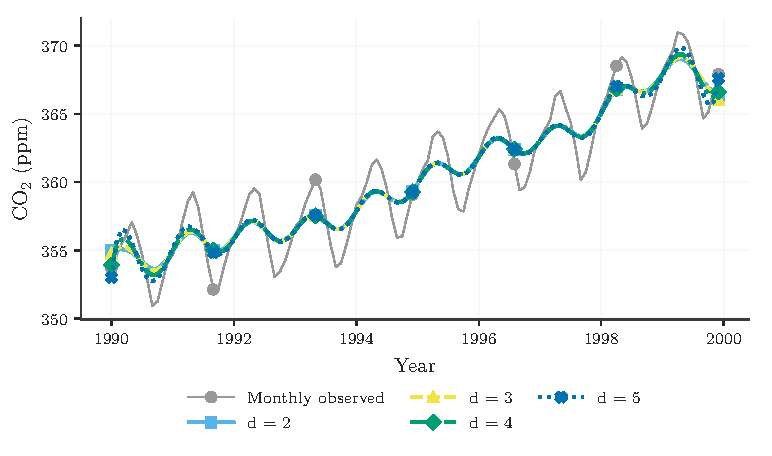
\includegraphics{figures/mauna_loa_1990_1999.pdf}
\caption{Historical Mauna Loa atmospheric carbon dioxide,
monthly aggregates of weekly measurements from 1990--1999,
and two-sided PLS fits with common normalized smoothness
$S=0.86$. These are descriptive trends, not forecasts.}
\label{fig:real-co2}
\end{figure}

The reference mean is fixed at $\mu=0$ for each displayed order,
so the curves show the effect of changing $d$ while keeping the
normalized trace-based smoothness index constant. This descriptive
comparison does not estimate $\mu$ from the data, optimize a Gaussian
marginal likelihood, or provide a forecast evaluation. The observed
seasonal fluctuations should not be interpreted as independent
measurement noise.

A full atmospheric analysis would explicitly model annual
seasonality, measurement uncertainty, and revisions to the
underlying data. The present package smooths the complete
observed series; it does not estimate predictive skill from
future held-out years.
